\begin{abstractbook}
\textbf{\begin{center}Abstract\end{center}}
Caution : You need to give an English Abstract by begin-abstractbook.This is a template for SJTU speech lab tech reports.
\end{abstractbook}

\section{Things to keep in mind}
\label{sec:intro}
%\usepackage{indentfirst}
%\setlength{\parindent}{2em} 
You are required to use English, unless you are writing a prose or something that requires literature skills.

Please do 'svn update' everytime before you edit.

We, editors, will only include your 'tech.tex' file.

Please use '\textbackslash input' to include child file, not '
\textbackslash include'.

Plase put '\textbackslash bibliography{\textbackslash ppath/ref}' in main.tex\cite{sjtuTech}.

Please submit a minimal ref.bib, and make sure that your ref terms won't coincide with others. You can use your id as a prefix of ref terms.

Important, when you need to write a path, use '\textbackslash ppath' as the prefix in the path, as in the exmaple figure below, instead of '.'.

\begin{figure}[htbp]
\centering
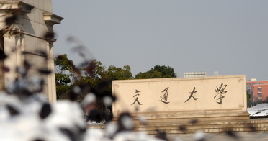
\includegraphics[width=14cm]{\ppath/figures/abc.png}
%\caption{this is graphic}
\label{fig:abc}
\end{figure}

If you want to add some code, use '\textbackslash lstlisting', below is C
\begin{lstlisting}[language=C]
#include<stdio.h>
int main() {
	printf("I love TechReports.\n");
}
\end{lstlisting}
below is bash
\begin{lstlisting}[language=bash]
echo I love TechReports.
\end{lstlisting}
